%--------------------------------------------------------
% style 
%--------------------------------------------------------

\documentclass[11pt, a4paper]{article}

\usepackage{epsfig}
\usepackage{subfigure}
\usepackage{graphicx}

\usepackage{ifpdf}
\ifpdf
\usepackage{epstopdf}
\usepackage[usenames,dvipsnames]{color}
\usepackage[pdftex,bookmarks=true,hypertexnames=false]{hyperref}
\hypersetup{
  pdfauthor = {Daniel Lenz, Jing Liu},
  pdftitle = {GSTR_08-M007},
  pdfsubject = {Pulse shape simulation},
  pdfkeywords = {Pulse shape simulation, germanium detector},
}
\pdfadjustspacing=1
\else
\usepackage[usenames,dvips]{color}
\fi

\setlength{\oddsidemargin}{0cm}
\setlength{\evensidemargin}{0cm}
\setlength{\topmargin}{-1cm}
\setlength{\textheight}{23cm}
\setlength{\textwidth}{16cm}

\pagestyle{headings}

\newcommand{\mage}     {{\sc MaGe}}
\newcommand{\geant}    {{\sc GEANT4}}
\newcommand{\rootv}    {{\sc ROOT}}
\newcommand{\gerda}    {{\sc GERDA}}
\newcommand{\majorana} {{\sc Majorana}} 
\newcommand{\decay}   {{\sc DECAY0}}
\newcommand{\eqref}[1]{Eq.\,(\ref{#1})}
\newcommand{\eqsref}[2]{Eqs.\,(\ref{#1}),\,(\ref{#2})}
\newcommand{\figref}[1]{Fig.\,\ref{#1}}
\newcommand{\figsref}[2]{Figs.\,\ref{#1},\,\ref{#2}}
\newcommand{\cms}{c.m.\,}
 
%--------------------------------------------------------

\begin{document}

% -------------------------------------------------------- 
% title 
% -------------------------------------------------------- 

\begin{titlepage}

\begin{figure}
\leftline{ \epsfig{file=GERDA-Logo.eps,width=0.15\textwidth}
\hspace{3.2 cm} 
GERDA Scientific / Technical Report: GSTR-08-M007}
\end{figure} 

\hspace{10.8cm} August 14th 2008 \\ 

\begin{center}

\vspace{1.0cm}

{\Large Pulse Shape Simulation and Analysis\\ } 

\vspace{0.5cm} 

%{\large \\ }

\vspace{1.0cm}

{\large 
Daniel Lenz, Jing Liu
}

\vspace{1.0cm}

{\it 
Max-Planck-Institut f\"ur Physik, M\"unchen, Germany
} 
\vspace{2.0cm} 
\begin{abstract}
  This note contains 1. a detailed documentation of the pulse shape   simulation codes, 2. some basic verifications of the simulation   codes, and 3. some simple applications of the simulation.
\end{abstract}
\end{center} 

\end{titlepage} 

% -------------------------------------------------------- 
% table of contents 
% -------------------------------------------------------- 

\pagenumbering{roman}

\tableofcontents

\pagebreak \setcounter{page}{1} \pagenumbering{arabic}

% -------------------------------------------------------- 
% main body 
% -------------------------------------------------------- 

\section{Documentation of the simulation package}
\label{sec:manual}
\subsection{Calculation of the charge carriers drift velocities}
\label{sec:drift}
Following a $\gamma$-ray interaction, the produced electron-hole pairs will separated and start to drift under the influence of the electrostatic field produced by the potential applied on the detector electrodes. One can define the mobility $\mu_{e,h}$ of the electrons $e$ and holes $h$ as the variable which gives the relation between the electric field $\mathbf{E}(\mathbf{r})$ and the drift velocity
\begin{equation}
  \label{eq:mobi}
  \mathbf{v}(\mathbf{r}) = \mu_{e,h} \mathbf{E}(\mathbf{r}),
\end{equation}
where $\mathbf{r}$ indicates the position. $\mu_{e,h}$ depend on the temperature, the electric field and the structure of the germanium crystal.

\subsubsection{Introduction}
\label{sec:drin}

\subsubsection{Electron drift velocity}
\label{sec:elec}
\begin{figure}[tbhp]
  \centering
  \includegraphics[width=0.4\textwidth]{valleys.eps}  
  \caption{Orientations of the crystal axes and valleys in the lab coordinate system XYZ.}
  \label{fig:valley}
\end{figure}

The dependence of the electron drift velocity $\mathbf{v}_{e}$ on the applied electric field $\mathbf{E}$ is taken to be
\begin{equation}
  \label{eq:ed}
  \mathbf{v}_{e}(\mathbf{E}) = \mathcal{A}(|\mathbf{E}|) \sum_{j} \frac{n_{j}}{n}     \frac{\gamma_{j}\mathbf{E_{0}}}     {\sqrt{\mathbf{E_{0}}\gamma_{j}\mathbf{E_{0}}}},  \mbox{ with }     j=1,2,3,4
\end{equation}
where $\mathcal{A}$ is a function of the magnitude of the electric field and temperature, the value of $\mathcal{A}$ must be negative because electrons drift to the opposite direction of the electric field; $\mathbf{E_{0}}$ is the normalized electric field vector; $n_{j}/n$ is the fraction  of the carriers (in this case, electrons) in the $j$-th valley, $\gamma_{j}$ is the effective mass tensor for the $j$-th valley. In general the tensor $j$-th is given in terms of the rotation matrices $R_{i}$, responsible for aligning the $i$-th $\langle 111 \rangle$ axis with the Y-axis of the lab system, by
\begin{equation}
  \label{eq:gammas}
  \gamma_{j} = R_{j}^{T}\gamma_{0}R_{j}, \mbox{ with } \gamma_{0}   \equiv \left(
    \begin{array}{ccc}
      m_{t}^{-1} & 0 & 0 \\
      0 & m_{l}^{-1} & 0 \\
      0 & 0 & m_{t}^{-1}
    \end{array} \right),
\end{equation}
where $m_{t} = 1.64m_{e}, m_{l} = 0.0819m_{e}$ with $m_{e}$ denoting the free electron mass, and the rotation matrix $R_{j} = R_{x^{\prime}}(\arccos(\sqrt{2/3}))R_{z}((j-1)\pi/2)$.

\begin{figure}[tbhp]
  \centering
  \includegraphics[width=0.6\textwidth]{axes.eps}  
  \caption{Orientations of the crystal axes and valleys in the lab coordinate system XYZ.}
  \label{fig:axes}
\end{figure}

For an experimental determination of the repopulation amplitude, the deviation from a uniform population distribution $n_{e}/n$ (1/4 for germanium) is assumed to vary with the electric field weighted by the factor $\mathcal{R}$:
\begin{equation}
  \label{eq:nion}
  \frac{n_{j}}{n} = \mathcal{R(|\mathbf{E}|)}   \left[         \frac{\sqrt{\mathbf{E_{0}}\gamma_{j}\mathbf{E_{0}}}}
    {\sum_{i}\sqrt{\mathbf{E_{0}}\gamma_{i}\mathbf{E_{0}}}} -               \frac{n_{e}}{n} \right] + \frac{n_{e}}{n},  \mbox{ with }           i=1,2,3,4
\end{equation}

If the electric field vector is equally oriented with respect to all the $\langle111\rangle$ directions, there is an uniform repopulation of the conduction bands, \textit{i.e.} $n_{j}/n = 1/4$. An electric field applied along the $\langle100\rangle$ direction, \textit{i.e.} $\mathbf{E_{0}} = (1/\sqrt{2},1/\sqrt{2},0)^{T}$, satisfies this condition. By employing the experimental drift velocity $v_{e}^{exp}(E)$ for an applied electric field $E$ in the $\langle100\rangle$ direction at a specific temperature, the absolute value  of $\mathcal{A}(|\mathbf{E}|)$ can be calculated as
\begin{equation}
  \label{eq:ae}
  \mathcal{A}(|\mathbf{E}|) = \frac{v_{e}^{exp}(E)}  {\displaystyle \sum_{j}     \frac{1}{4}     \frac{\gamma_{j}\mathbf{E_{0}}}         {\sqrt{\mathbf{E_{0}}\gamma_{j}\mathbf{E_{0}}}} },  \mbox{ with }       \mathbf{E_{0}} = \left( \begin{array}{c} 
    1/\sqrt{2}\\1/\sqrt{2}\\0 \end{array} \right).
\end{equation}

If the electric field vector is oriented along with one of the $\langle111\rangle$ directions, \textit{i.e.} $\mathbf{E_{0}} = (0,\sqrt{2}/\sqrt{3},1/\sqrt{3})^{T}$, there is an uniform repopulation of the conduction bands among the other three $\langle111\rangle$-axes, \textit{i.e.}
\begin{equation}
  \label{eq:n111}
  \frac{n_{2}}{n} = \frac{n_{3}}{n} = \frac{n_{4}}{n}.
\end{equation}
Since
\begin{equation}
  \label{eq:nsum}
  \displaystyle \sum_{j}\frac{n_{j}}{n} = 1,
\end{equation}
we have
\begin{equation}
  \label{eq:n12}
  \frac{n_{1}}{n} + 3\frac{n_{2}}{n}= 1.
\end{equation}
By employing the experimental drift velocity $v_{e}^{exp}(E)$ for an applied electric field $E$ in the $\langle111\rangle$ direction at a specific temperature, we have another relation between $n_{1}/n$ and $n_{2}/n$:
\begin{equation}
  \label{eq:n12p}
  v_{e}^{exp}(E) =  \mathcal{A}(|\mathbf{E}|) \left(  \frac{n_{1}}{n} \frac{\gamma_{1}\mathbf{E_{0}}}         {\sqrt{\mathbf{E_{0}}\gamma_{1}\mathbf{E_{0}}}} +  3\frac{n_{2}}{n} \frac{\gamma_{2}\mathbf{E_{0}}}         {\sqrt{\mathbf{E_{0}}\gamma_{2}\mathbf{E_{0}}}} \right).
\end{equation}
One can get the value of $n_{1}/n$ and $n_{2}/n$ by solving the equations \ref{eq:n12} and \ref{eq:n12p} together. Then $\mathcal{R}(|\mathbf{E}|)$ can be calculated as
\begin{equation}
  \label{eq:re}
  \mathcal{R(|\mathbf{E}|)} = \left( \frac{n_{1}}{n} - \frac{n_{e}}{n}     \right) / \left(     \frac{\sqrt{\mathbf{E_{0}}\gamma_{1}\mathbf{E_{0}}}}
    {\sum_{i}\sqrt{\mathbf{E_{0}}\gamma_{i}\mathbf{E_{0}}}} -                           \frac{n_{e}}{n} \right),  \mbox{ with }           i=1,2,3,4 \mbox{ and       } \mathbf{E_{0}} = \left( \begin{array}{c} 
      0\\ \sqrt{2}/\sqrt{3}\\1/\sqrt{3} \end{array} \right).
\end{equation}

The dependence of the experimental $\langle111\rangle$ and $\langle100\rangle$ drift velocities on the electric field can be fitted with the empirical formula: 
\begin{equation}
  \label{eq:expe}  
  v_{e}^{exp}(E) = \frac{\mu_{0}E}{(1+(E/E_{0})^{\beta})^{1/\beta}} - \mu_{n}E.
\end{equation}
The fitted parameters values are presented in Table~\ref{tab:pare}
\begin{table}[tbhp]
  \centering
  \begin{tabular}{ccccc}\hline\hline
    Direction & $\mu_{0} \left[ \frac{\mbox{cm}^{2}}{\mbox{V}\cdot\mbox{s}} \right]$ & $E_{0} \left[ \frac{\mbox{V}}{\mbox{cm}} \right]$ & $\beta$ & $\mu_{n} \left[ \frac{\mbox{cm}^{2}}{\mbox{V}\cdot\mbox{s}} \right]$ \\\hline
$\langle111\rangle$ & 40180 & 493 & 0.72 & 589 \\
$\langle100\rangle$ & 42420 & 251 & 0.87 & 62\\ \hline\hline
  \end{tabular}
  \caption{Fit parameters for the experimental drift velocities in the 
$\langle111\rangle$ and $\langle100\rangle$ directions.}
\label{tab:pare}
\end{table}

After determination of the parameters $\mathcal{A}$ and $\mathcal{R}$, the drift velocity can be calculated for any direction and any strength of the electric field.

\subsubsection{Hole drift velocity}
\label{sec:hole}
The three components $(v_{x^{\prime}}, v_{y^{\prime}}, v_{z^{\prime}})^{T}$ of the hole drift velocity $\mathbf{v}$ in the local coordinate $x^{\prime}y^{\prime}z^{\prime}$ (as shown in Fig.~\ref{fig:vsphere}) can be expressed as:
\begin{equation}
  \label{eq:vsphere}
  \begin{array}{rcl}
   v_{x^{\prime}} = v_{r} &=& v_{100}(E)[1-\Lambda(k_{0})(\sin(\theta)^{4}\sin(2\phi)^{2} + \sin(2\theta)^{2})]\\
   v_{y^{\prime}} = v_{\theta} &=& v_{100}(E)\Omega(k_{0})[2\sin(\theta)^{3}\cos(\theta)\sin(2\phi)^{2} + \sin(4\theta)]\\
    v_{z^{\prime}} = v_{\phi} &=& v_{100}(E)\Omega(k_{0})\sin(\theta)^{3}\sin(4\phi)
  \end{array}
\end{equation}
\begin{figure}[tbhp]
  \centering
  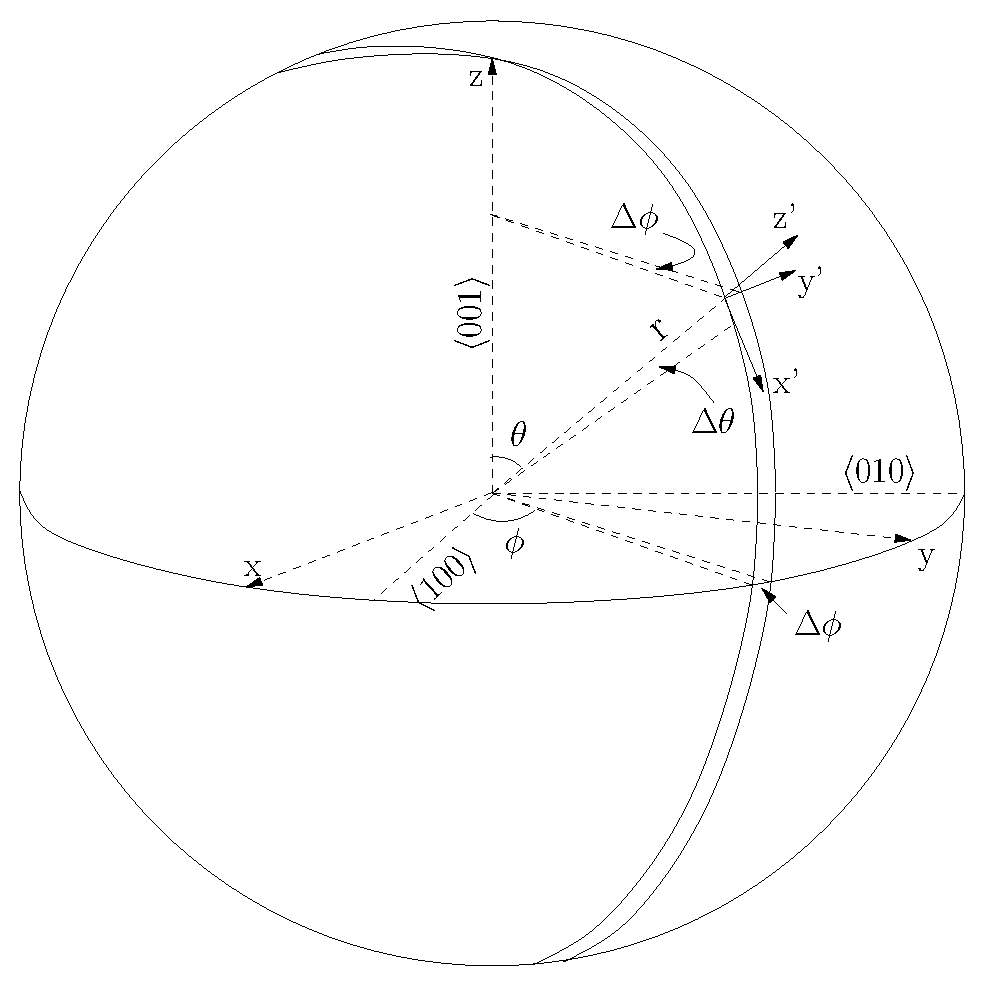
\includegraphics[width=0.6\textwidth]{vsphere.eps}  
  \caption{Orientations of the crystal axes and valleys in the lab
coordinate system XYZ.}
  \label{fig:vsphere}
\end{figure}
The mean wave number $k_{0}$ can be expressed as a function of $v_{rel} = v_{111}/v_{100}$:
\begin{equation}
  \label{eq:k0}
   k_{0}(v_{rel}) = 9.2652 - 26.3467v_{rel} + 29.6137v_{rel}^{2} - 12.3689v_{rel}^{3}
\end{equation}
The function $\Lambda$ and $\Omega$ govern the amplitude of the anisotropy and can be expressed as
\begin{equation}
  \label{eq:lamb}
   \Lambda(k_{0}) = -0.01322k_{0} + 0.41145k_{0}^{2} - 0.23657k_{0}^{3} + 0.04077k_{0}^{4}
\end{equation}
\begin{equation}
  \label{eq:ome}
   \Omega(k_{0}) = 0.006550k_{0} - 0.19946k_{0}^{2} + 0.09859k_{0}^{3} - 0.01559k_{0}^{4}
\end{equation}
The dependence of the experimental $\langle111\rangle$ and $\langle100\rangle$ drift velocities, \textit{i.e.} $v_{111}$ and $v_{100}$ on the electric field can be fitted with the empirical formula: 
\begin{equation}
  \label{eq:exph}  
  v_{h}^{exp}(E) = \frac{\mu_{0}E}{(1+(E/E_{0})^{\beta})^{1/\beta}}.
\end{equation}
The fitted parameters values are presented in Table~\ref{tab:parh}
\begin{table}[tbhp]
  \centering
  \begin{tabular}{cccc}\hline\hline
    Direction & $\mu_{0} \left[ \frac{\mbox{cm}^{2}}{\mbox{V}\cdot\mbox{s}} \right]$ & $E_{0} \left[ \frac{\mbox{V}}{\mbox{cm}} \right]$ & $\beta$ \\\hline
$\langle111\rangle$ & 107270 & 0.580 & 100 \\
$\langle100\rangle$ & 66333 & 0.744 & 181 \\ \hline\hline
  \end{tabular}
  \caption{Fit parameters for the experimental drift velocities in the 
$\langle111\rangle$ and $\langle100\rangle$ directions.}
\label{tab:parh}
\end{table}

The three components $(v_{x}, v_{y}, v_{z})^{T}$ of the hole drift velocity $\mathbf{v}$ in the lab coordinate $xyz$ (as shown in Fig.~\ref{fig:vsphere}) can be calculated as:
\begin{equation}
  \label{eq:v2v}  
  \left(
    \begin{array}{c}
      v_{x} \\ v_{y} \\ v_{z}
    \end{array}
\right) = R_{z}(\phi + \frac{\pi}{4} + \phi_{110}) R_{y^{\prime}}(\theta) \left( 
    \begin{array}{c}
      v_{x^{\prime}} \\ v_{y^{\prime}} \\ v_{z^{\prime}}
    \end{array} \right)
\end{equation}

%%% Local Variables:
%%% mode:latex
%%% TeX-master: "GSTR-08-M007"
%%% End:

\subsection{Calculation of the electric fields and potentials}
\label{sec:field}




%%% Local Variables:
%%% mode:latex
%%% TeX-master: "GSTR-08-M007"
%%% End:


\section{Verification of the simulation}
\label{sec:verify}


\section{Pulse shape analysis}
\label{sec:physics}


\clearpage
 
\begin{thebibliography}{sotief}

%\cite{Abt:2004yk}
%\bibitem{Abt:2004yk} 

\end{thebibliography}


\end{document}

